\PassOptionsToPackage{hidelinks}{hyperref}
\documentclass[doc,biblatex]{apa7}
\DeclareLanguageMapping{american}{american-apa}
\addbibresource{references.bib}
\captionsetup[figure]{textfont=rm,font=small,labelfont=bf}
\usepackage{amsmath}
\usepackage{mathspec}
\setallmainfonts{Times New Roman}
\setmainfont{Times New Roman}
% \setsansfont{Helvetica Neue}


\title{Why do languages tolerate heterography? An experimental investigation of the cultural evolution of informative orthography}

\shorttitle{The cultural evolution of informative orthography}

\authorsnames[1,1]{Jon W. Carr, Kathleen Rastle}

\authorsaffiliations{{Department of Psychology, Royal Holloway, University of London, England}}

% \authornote{\textbf{Cite as:} Carr, J.\@ W., \& Rastle, K.\@ (2023). Informativity in the writing system. \textit{OSF Preprints}. Version~0.}

\abstract{It is widely acknowledged that opaque orthographies place additional demands on learning, often requiring many years to acquire fully. It is less widely recognized, however, that such orthographies may offer certain benefits in the context of reading. For example, the heterographic homophones (e.g., <knight> vs. <night>) impose additional costs in learning but reduce ambiguity in reading. Could it be the case, then, that heterography---and therefore orthographic opacity---may sometimes be selected for in the evolution of writing systems, despite the cost in learning? We investigate this question by simulating the evolution of orthography as it is transmitted from one generation to the next, both with and without a communicative pressure for avoiding ambiguity. In addition, we consider two mechanisms by which informative heterography might be selected for: \textit{differentiation}, in which new spellings are created to differentiate words that are homophonous in speech (e.g., <lite> from <light> to signal low-fat), and \textit{conservation}, in which heterography arises through exaptation as an epiphenomenon of sound change (e.g., <meat> vs. <meet> resulting from the /ɛː/–/eː/ merger in the Great Vowel Shift). Under pressure from learning alone, orthographic systems become transparent, but when combined with communicative pressure, these systems can become informative, diverging from the spoken language in order to express meaning directly.}

\keywords{communication; cultural evolution; informativity; iterated learning; language evolution; orthography; spelling; sound change; writing}

\begin{document}

\maketitle

\noindent
Written languages represent spoken languages. However, there are many ways in which written languages diverge. E.g. spacing between words helps readers parse a sentence even if they are not technically required. Written languages can also have there own regularities such as spelling related words similarly (magician), past tense spellings directly conveying meaning, certain spellings conveying word class ous. These features abound in writing, especially in languages such as English that have not been subject to serious regulation.

One notable case of this is the heterographic homophones---words that sound alike but which are written with different spellings. For example, <meat> and <meet> are both pronounced /miːt/. Furthermore, these spellings can be cognitively useful . For example, faced with a sentence beginning /ðɛr/, a listener will have high uncertainty about what word---or even what sentence structure---is likely to come next: a noun, as in /ðɛr dɒg/, a form of the verb to be, as in /ðɛr ɪz/, or the progressive form of a verb, as in /ðɛr gəʊɪŋ/. In writing, by contrast, this uncertainty is greatly reduced; the spellings <their>, <there>, and <they're> differentiate between these cases, giving the reader a headstart on parsing the upcoming syntax. This idiosyncratic spelling of words that are homophonous in speech may confer certain benefits in reading, particularly in terms of comprehension. Heterography permits a writing system to be---at least in some areas---more informative than its spoken counterpart.

Other languages

Irish orthography has special features to handle lenition and eclipsis. For example, when the word /pɑʃti/ (children) is eclipsed, it becomes /bɑʃti/ (the initial consonant is vocalized), but the spelling system retains the letter <p> in addition to adding a <b>: <páistí> becomes <bpáistí> under eclipsis. This allows the reader quick access to the root word from which the eclipsed form is derived and, in some cases, results in ambiguity avoidance (in this case, if the <p> were not retained, the spelling <báistí> would be confusible with the word for rain).

However, this additional informativeness comes at a cost. A system of words that conveys more information will---in general---be more complex than one that conveys less information. There exists a tradeoff between the simplicity of the spelling system and its ability to be expressive. A simple spelling system is one that is easy to learn, use, and process; for example, by being transparent with respect to phonology. The idea of a tradeoff between simplicity and informativeness in language structure has a longstanding history \parencite{Gabelentz:1891, Zipf:1949, Martinet:1952, Rosch:1978} and has recently been explored in a wide range of both typological \parencite{KempRegier:2012, Kemp:2018} and experimental \parencite{Carr:2020, Kirby:2015} studies. Of particular note here is the idea that the pressure for simplicity in language structure derives principally from learning, while the pressure for informativeness derives from the need for precise communication.

Any explanation for heterographic homophones must, therefore, demonstrate that heterographic spellings convey a benefit in terms of informativeness that is outweighed by the cost of learning the (often arbitrary) spelling distinction. What are the benefits? There seem to be broadly two kinds of benefit. (1) disambiguation in the writing of words that would otherwise be ambiguous if spelled transparently. (2) permitting the cognitive system to rapidly and accurately attain the meaning of a word. In this paper we limit ourselves to informativeness of the first kind, which is more amenable to experimental testing.

Is it possible, then, that heterography may be selected for in the cultural evolution of orthography? And if so, what might be the mechanism through which such selection could operate? \textcite[pp.~325--326]{Berg:2021} sketch two models of how a word might enter a state of heterography, as depicted in Fig.~\ref{models_of_heterography}. The first model, \textit{the differentiation model}, explains heterography through the creation of a new orthographic forms. For example, the word \textit{lite} is a respelling of \textit{light} frequently used in food products to distinguish light-in-calorific-weight from other meanings of \textit{light}; in British English, the word \textit{cheque} (perhaps influenced by \textit{exchequer}) differentiates the bank draft from other meanings of the word \textit{check}; and the word \textit{byte} was a deliberate respelling of \textit{bite} to avoid accidental mutation into the closely related term \textit{bit} \parencite{Buchholz:1977}. Etymological (and folk-etymological) spellings introduced during the Renaissance also occasionally resulted in heterographic homophones, perhaps contributing to their success: \textit{scene}--\textit{seen}, \textit{scent}--\textit{sent}, \textit{whole}--\textit{hole} \parencite[pp.~58--59]{Scragg:1974}, and many monosyllabic words that are homophonous with common function words have tended to adopt alternate spellings: \textit{be}--\textit{bee}, \textit{but}--\textit{butt}, \textit{by}--\textit{bye}--\textit{buy}, \textit{for}--\textit{fore}--\textit{four}, \textit{in}--\textit{inn}, \textit{or}--\textit{oar}--\textit{ore}, \textit{so}--\textit{sew}, \textit{to}--\textit{too}--\textit{two}, etc. Heterography is also very common in proper nouns: Surnames that are homophonous with common nouns often add <e> (\textit{Clarke}, \textit{Greene}, \textit{Wilde}) or double the final consonant (\textit{Carr}, \textit{Hogg}, \textit{Mann}), and it is common for brand names to adopt creative spellings, such as \textit{flickr}, \textit{Froot Loops}, or \textit{MVMT}.

	\begin{figure}
	\makebox[\textwidth][c]{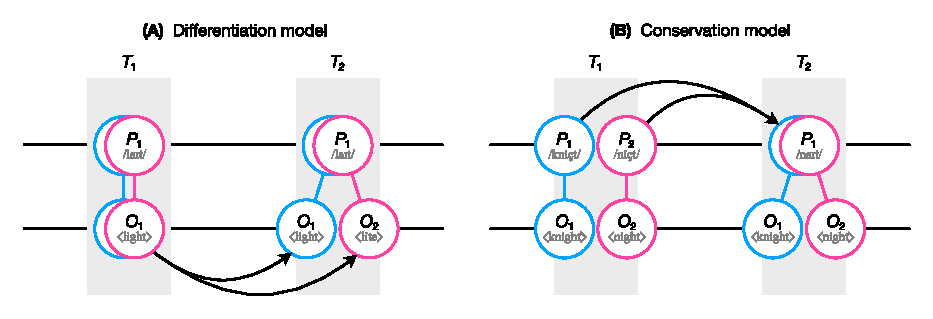
\includegraphics[]{figs/models_of_heterography.eps}}
	\vspace*{2pt}
	\caption{Two models of heterography. In the differentiation model, two meanings (represented by pink and blue) are, at time $T_1$, expressed by a single phonetic form $P_1$ and a single orthographic form $O_1$; however, by time $T_2$, two orthographic forms have emerged to differentiate the meanings in writing. In the conservation model, the two distinct phonetic forms that existed at time $T_1$ have become homophonous by time $T_2$, but the two corresponding orthographic forms have been conserved, resulting in the same state of heterography as in the differentiation model. Adapted from \textcite[pp.~325--326]{Berg:2021} with permission.}
	\label{models_of_heterography}
	\end{figure}

The second model, \textit{the conservation model}, explains heterography as the historical residue of sound change: Two (or more) spoken forms merge and become homophonous, but the original heterographic spellings are conserved in the orthography. In English, for example, the meat--meet merger ultimately resulted in Middle English /ɛ:/ (spelled <ea>) and /e:/ (spelled <ee>) merging into /i:/ in Early Modern English, although the spellings were never updated accordingly, thus giving rise to a set heterographic homophones that persist in present-day English: \textit{heal}--\textit{heel}, \textit{leak}--\textit{leek}, \textit{meat}--\textit{meet}, \textit{read}--\textit{reed}, \textit{sea}--\textit{see}, \textit{team}--\textit{teem}, \textit{weak}--\textit{week}, etc. Similarly, other historic sound changes have likely resulted in (or contributed to) pairs of words entering a state of heterography, such as the reduction of /kn/ into /n/ (\textit{knight}--\textit{night}, \textit{know}--\textit{no}, \textit{knot}--\textit{not}, etc.), the loss of /ç/ (\textit{eight}--\textit{ate}, \textit{right}--\textit{rite}, \textit{sight}--\textit{site}, etc.), and the merger of /ʍ/ into /w/ (\textit{whale}--\textit{wail}, \textit{which}--\textit{witch}, \textit{whine}--\textit{wine}, etc.).

Processes

Sound change
dialect merger (bury is the spelling from one dialect with the pronunciation from another dialect)
Borrowing (English tends to retain spelling from the source language)
Printers innovations
- Etymological spellings (doubt)
- Deliberate design of heterographs
- Morphological spellings

\subsection{Research questions}

Q1) Does a learning pressure (induced through cultural transmission) result in the emergence of a simple, systematic, transparent orthography that is easier to learn? Hypotheses: In the high-variation conditions, where the orthography starts out chaotic (resulting in holistic systems), we expect simpler systems to emerge. Simplicity may be realized in a number of ways. Transparent systems use a one-to-one mapping to directly represent the spoken forms in writing. Redundant systems retain some spelling variation (with idiosyncratic spellings of the suffix for each shape) but become simpler by collapsing across colour. Expressive systems continue to express colour, but do so with a non-transparent but easy to learn compositional suffix system. The prevalence of these three types of system will be influenced by the presence of the communicative pressure. When communication is not present, transparent systems will tend to dominate, alongside some redundant systems and possibly some expressive systems. When communication is present, expressive systems will tend to dominate, perhaps with some redundant and holistic forms. The gradual emergence of simplicity, whatever form it takes, should be accompanied by increased learnability.

Q2) Can a writing system evolve to become more informative than its uninformative spoken counterpart? Hypotheses: Yes, but preferentially when two vital ingredients are present: a communicative pressure for informativeness (which makes an expressive system desirable) and high variation (which provides the building blocks to make that happen). When both ingredients are present, expressive systems will tend to dominate. If only one of the ingredients is available (either communication or high variation), informative systems may emerge but are less likely. In the case of learning-only and high-variation, expressive systems may emerge if the learners – yearning for an explanation for the variation – assume that colour must somehow be involved and therefore impose (perhaps unconsciously) colour-expressive structure on the language (i.e. learners may, to a certain extent, have a preconceived notion that languages ought to be informative). In the case of communication and no variation (where, again, only one of the ingredients is met), expressive systems may emerge but this is highly dependent on participants being 'innovators' who are willing to develop novel spelling systems that diverge from the spoken system in order to express colour. If neither ingredient is present, expressive systems will not emerge.



%~%~%~%~%~%~%~%~%~%~%~%~%~%~%~%~%~%~%~%~%~%~%~%~%~%~%~%~%~%~%~%~%~%~%~%~%~%~%~%~%~%~%~%~%~%~%~%~%~%~%~%

\section{Experiment 1}

Our first experiment tests the ability of the differentiation model to explain the emergence of informativeness in orthography. In particular we had two main hypotheses:


Preregistered \url{https://aspredicted.org/YLG_CKD}

\subsection{Methods}

To simulate the cultural evolution of orthography, we adopt the experimental iterated learning paradigm \parencite{Kirby:2008, Kirby:2015}. In this paradigm, some linguistic system is passed along a \textit{transmission chain} of human participants, resulting in repeated cycles of learning and production. Participant $i$ in a transmission chain learns the system based on the linguistic output of participant $i-1$ and then produces new linguistic output for participant $i+1$ to learn from. Following several \textit{generations} of this process, the linguistic system can gradually adapt to the learning biases of the human learners, yielding interesting emergent phenomena, such as compositionality \parencite{Kirby:2008, Kirby:2015}, combinatoriality \parencite{Verhoef:2015}, category structure \parencite{Carr:2017, Carr:2020}, and regularization \parencite{Smith:2010, Ferdinand:2019}. To explore the hypotheses outlined above, we conducted the experiment under two conditions: Transmission-only and Transmission~+ Communication.

\subsubsection{Participants}

We recruited 287 participants via the Prolific platform. Participants were paid £2.00 for participation plus additional bonuses of up to £1.08 as detailed below (median bonus: £0.74). The median completion time was 15~m with a median hourly rate of £8.05 (£10.94 including bonus). We limited recruitment to (self-declared) native English speakers, since it was important that participants would perceive the spoken forms in a relatively consistent way (particularly in the case of Experiment~2). 14 participants were excluded because they (or their partners) used English color words (8) or failed the auditory attention checks (6). A further three participants were lost to communication-game pairing failures. The final dataset comprises 270 participants: 90 in the Transmission-only condition (10 chains of 9 subjects) and 180 in the Transmission~+ Communication condition (10 chains of 9 pairs of subjects).

\subsubsection{Stimuli}

	\begin{figure}
	\makebox[\textwidth][c]{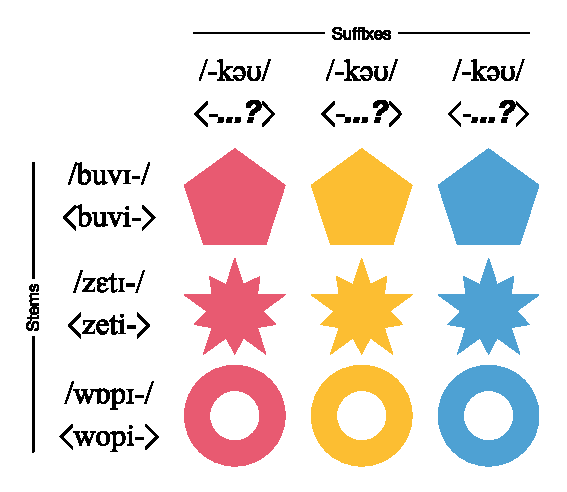
\includegraphics[]{figs/stimuli.eps}}
	\vspace*{2pt}
	\caption{The nine alien object stimuli with their iconic stems (indicating shape) and suffixes (indicating color). The spoken forms of the suffixes are homophonous, but their associated spellings are free to evolve and may therefore take on differentiated forms.}
	\label{stimuli}
	\end{figure}

Participants were taught words for nine ``alien'' objects---three shapes (pentagon, star, torus) in three colors (pink, yellow, blue), as depicted in Fig.~\ref{stimuli}. The alien words had a spoken and written form composed of a stem and suffix. The stems, which always express the shape dimension, were /buvɪ/ <buvi> (the pentagon), /zɛtɪ/ <zeti> (the star), and /wɒpɪ/ <wopi> (the torus). These stems were fixed and unchanging throughout both experiments reported in this paper and were designed to be easy to learn by being graphically and phonetically iconic of the shapes they represent. Throughout Experiment~1, the spoken form of the suffix was always pronounced /kəʊ/, but its spelling was free to change over time. Thus, the spoken form of the language consists of just three unique words---/buvɪkəʊ/, /zɛtɪkəʊ/, and /wɒpɪkəʊ/---that mark only a shape distinction; however, the spelling of the suffix could potentially take on different forms to mark color.

Each of the 10 transmission chains was seeded with a randomly-generated suffix spelling system. This was created by randomly mapping the following nine spellings onto the nine objects: <co>, <coe>, <coh>, <ko>, <koe>, <koh>, <qo>, <qoe>, <qoh>. In other words, the /k/ sound may be spelled <c>, <k>, or <q> and the /əʊ/ sound may be spelled <o>, <oe>, or <oh>, although the initial seed system contains no particular regularity. This models an initial state of high spelling variation (every object has a unique suffix spelling), which may, over time, become transparent (the /k/ and/or /əʊ/ sounds take on consistent spellings) or expressive (spellings of /k/ and/or /əʊ/ become systematically associated with meaning). The spoken forms were synthesized using the Apple text-to-speech synthesizer (Tessa voice).

\subsubsection{Transmission procedure}

	\begin{figure}
	\makebox[\textwidth][c]{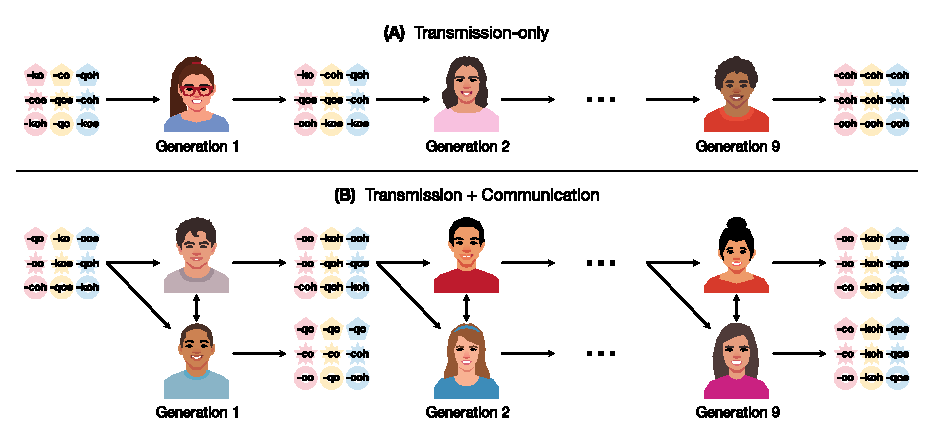
\includegraphics[]{figs/transmission.eps}}
	\vspace*{2pt}
	\caption{(A) Transmission-only procedure. Each generation consists of a single participant, who first receives training on six of the nine suffixes and then produces suffixes for all nine items. These productions are then used as the training material for the next generation in the chain. The initial system of suffixes is randomly generated with high spelling variation; but by the ninth generation, the system is expected to become transparent. (B) Transmission~+ Communication procedure. Each generation now consists of two participants who engage in a communicative task. Both participants receive training on the same system from the previous generation. Under a communicative pressure, the suffix spellings are expected to become expressive of color, despite the spoken forms being homophonous.}
	\label{transmission}
	\end{figure}

As outlined above, the participants were arranged into transmission chains such that the spellings produced by one participant would subsequently be taught to the next participant in the chain (see Fig.~\ref{transmission}A). The first participant in a chain was taught the initial, randomly generated seed system, and this system was then free to evolve as it was culturally transmitted. Importantly, this process was subject to a bottleneck on transmission: Not all nine spellings were transmitted from one generation to the next; rather, the participant at generation $i$ would observe only six of the nine spellings generated at generation $i-1$ (at least one of each shape and at least one of each color). Nevertheless, participants were asked to produce a spelling for all nine objects, meaning that generalization was required for three unseen items. Transmission continued for nine generations in each of ten independent chains. In the Transmission~+ Communication condition (see Fig.~\ref{transmission}B), each generation consists of a pair of participants, but the productions of only one of the participants (the primary participant) are iterated to the next generation (the productions of the secondary participant are thus a cultural deadend). The role of the secondary participant is to act as a communicative partner for the primary participant, inducing pressure for the language to become informative.

\subsubsection{Training procedure}

All participants were trained on the spoken and written forms through a combination of passive exposure trials and ``mini-test'' trials. Participants were also told explicitly that the stems were iconic of the objects' shapes, allowing participants to focus on learning the suffixes during the training phase. In passive exposure trials, the alien objects were presented alongside the written and spoken forms in quick succession for 2~s each. In mini-test trials, which were interleaved among the passive exposure trials, the participant was asked to type in the appropriate written form for an object and was given feedback on any errors (deleted characters shown in red strikethrough text and additions shown in bold green text). The participant received a 2p bonus for spelling the word correctly but had to submit their response within 20~s. Each of the six object--word pairs in the training set (i.e., the seen items that passed through the bottleneck on transmission) was passively exposed 18 times and mini-tested six times, resulting in a total of 108 passive exposure trials and 36 mini-test trials (the maximum bonus in training was therefore 72p). To check that participants were listening to the spoken forms, they were asked auditorily to click on the alien object at three random points during training; participants who did not follow this instruction were excluded.

\subsubsection{Test procedure in Transmission-only}

After training, participants assigned to the Transmission-only condition completed a test phase, alternating between production and comprehension trials. In production trials, the participant was shown an object and heard its associated word pronounced aloud. The participant's task was to type~in the appropriate spelling. The input box was limited to eight lowercase Latin characters, and participants had to spell the stem correctly to continue to the next trial. Since participants heard the word pronounced aloud, typing the stem correctly should have been trivial, but in cases where the stem was initially spelled incorrectly, a popup message explicitly reminded the participant of the correct spelling of the stem. This restriction was imposed to prevent the stems from diverging from their spoken forms over time; however, no such restriction was imposed on the spelling of the suffix. Since the overall word length was restricted to eight characters and since all stems were four letters long, participants could use, at a minimum, a zero suffix and, at a maximum, a four-letter suffix. In comprehension trials, the participant was shown a word and had to click on the matching object from an array of all nine objects arranged in random order (in cases where multiple objects were described by the same wordform, any of the objects was a valid choice). In both types of test trial, the participant was awarded a bonus of 2p for each correct answer, but no explicit feedback was provided. Each of the nine object--word pairs (i.e., including unseen items) was tested once in production and once in comprehension, resulting in 18 trials (the maximum bonus in test was therefore 36p).

\subsubsection{Test procedure in Transmission~+ Communication}

Participants assigned to the communicative condition completed a live, over-the-internet communication game with another participant, who had received training on the same orthographic system inherited from the previous generation (albeit on an independently selected set of seen items). The game closely mirrored the overall structure of the test administered to participants in the non-communicative condition, with the production and comprehension trials becoming the two sides of a single communicative interaction. On a given trial, one participant (the director) would complete a production trial under the same input restrictions described above (i.e., produce a form for a target meaning), and the word they used was relayed to the other participant (the matcher), who would then complete a comprehension trial in response to that word (i.e., pick an object from the matcher array). The two participants then switched roles, resulting in the same overall trial structure as the Transmission-only condition (i.e., alternation between production and comprehension trials and the same bonusing scheme).

The framing and goal of the communication game was, however, quite different from the non-communicative test. In communication, the shared goal of the director and matcher is to have a successful communicative interaction, not necessarily to reproduce what they had learned in training. Both participants received the 2p bonus each time an interaction was successful; that is, the reward structure is not based on using the ``correct'' forms taught in training but based on accurately conveying meaning. The director is thus incentivized to produce a wordform that is unambiguous, and the matcher is incentivized to carefully interpret what the director has attempted to convey. The second important difference from the non-communicative test was that participants received rich feedback on the interaction: The director saw which object the matcher clicked on, and the matcher saw which object was the correct target. Overall, then, the communication game is identical to the non-communicative test in terms of the task to be performed (nine productions and nine comprehensions), but the goal is quite different: In the non-communicative test, the goal and reward structure is based on accurately reproducing the orthography learned during training, whereas in the communication game, the goal and reward structure is based on successfully communicating a target object.

\subsection{Results}

	\begin{figure}
	\makebox[\textwidth][c]{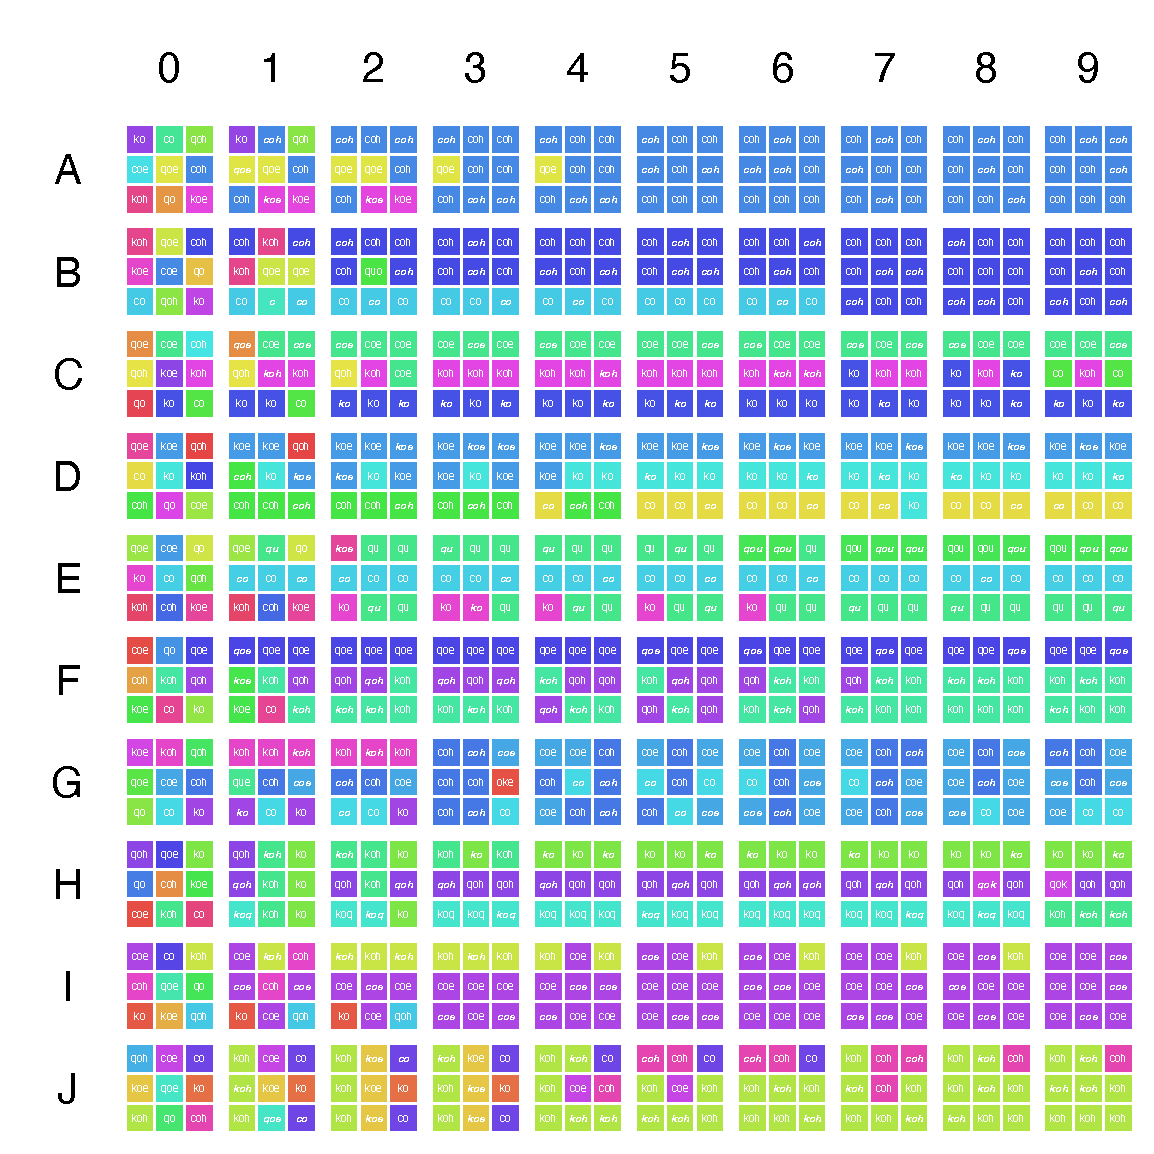
\includegraphics[]{figs/dif_lrn.eps}}
	\vspace*{2pt}
	\caption{Results from the Transmission-only condition in Experiment~1 (differentiation). Each matrix shows the suffix spelling system in use at a particular generation (shape on the rows, color on the columns, as in Fig.~\ref{stimuli}). Chains are labeled A--J and generations are labeled 0–9 (0 is the randomly generated seed system). Each chain uses an independent color palette, with each color representing a particular suffix spelling; similar colors indicate similar spellings. Spellings in bold-italic are the generalizations on unseen items. By the ninth generation, most systems are degenerate (e.g., Chains~A, B, and~I), redundant (e.g., Chains~D, E, and~H), or a mixture of the two (e.g., Chain~F).}
	\label{dif_lrn}
	\end{figure}

The results from all ten chains (labelled A--J) in the Transmission-only condition are shown in Fig.~\ref{dif_lrn}. Each 3×3 matrix represents the suffix spelling system in use at a particular generation with shape down the rows and color along the columns, just as in Fig.~\ref{stimuli}. For example, the system at Generation~9 in Chain~D uses three spellings---<koe>, <ko>, and <co>---to express the shape dimension. We describe such a system as ``redundant'' because shape is always expressed by the stem, so the suffix spellings that emerged in this case therefore convey no additional information. Similar outcomes occurred in Chains~C, E, F, and~H and are characteristic of the Transmission-only condition. We also saw the emergence of fully transparent suffix spelling systems in Chains~A, B, I, and~J. Chain~I, for example, ultimately uses a single spelling, <coe>, to represent the /kəʊ/ sound; that is, the written suffix forms make no distinction between shapes or colors, just like the spoken language. Chain~G did not settle on a clear pattern, using <co>, <coe>, and <coh> somewhat interchangeably in the final generation, although there were some signs of a color-expressive system emerging in, for example, Generation~6, where yellow is consistently spelled <coh>, blue is consistently spelled <coe>, and pink uses both <co> and <coe>. The only other signs of color-expressive systems are H1, which was rapidly converted into a redundant system in subsequent generations, and J2, which ultimately degenerated towards transparency.

The results for the Transmission~+ Communication condition (Chains~K--T) are shown in Fig.~\ref{dif_com}. Like Transmission-only, degeneration to a single spelling by the ninth generation is a relatively common outcome (e.g., Chains~N, R, and~S and to a lesser extent Chains~L, M, and~O). In contrast, redundant, shape-expressive systems (as indicated by horizontal stripes) are relatively rare (e.g., K8, M6 and Q1--6). Instead, the presence of the communicative task appears to favor color-expressive systems, although these are far from common and often unstable. In particular, there are two main kinds of color-expressive system that emerge. The first are the generalization-based expressive systems: K5, M1, P5, and S2. In these cases, the participant tended to generalize their input in a way that is consistent with expressing color over shape. For example, in K5, pink was consistently spelled <ko> and blue was consistently spelled <co>. In the case of M1, color is expressed by the final vowel letters (<oe> for pink, <o> for yellow, and <oh> for blue) with the spelling of the /k/ sound conditioned on the stem (<buvic->, <zetik->, and <wopiq->). We note, however, that in all these cases the expressive system was not reciprocated by the participant's partner, resulting in low communicative accuracy, and not sustained or elaborated~on in subsequent generations.

	\begin{figure}
	\makebox[\textwidth][c]{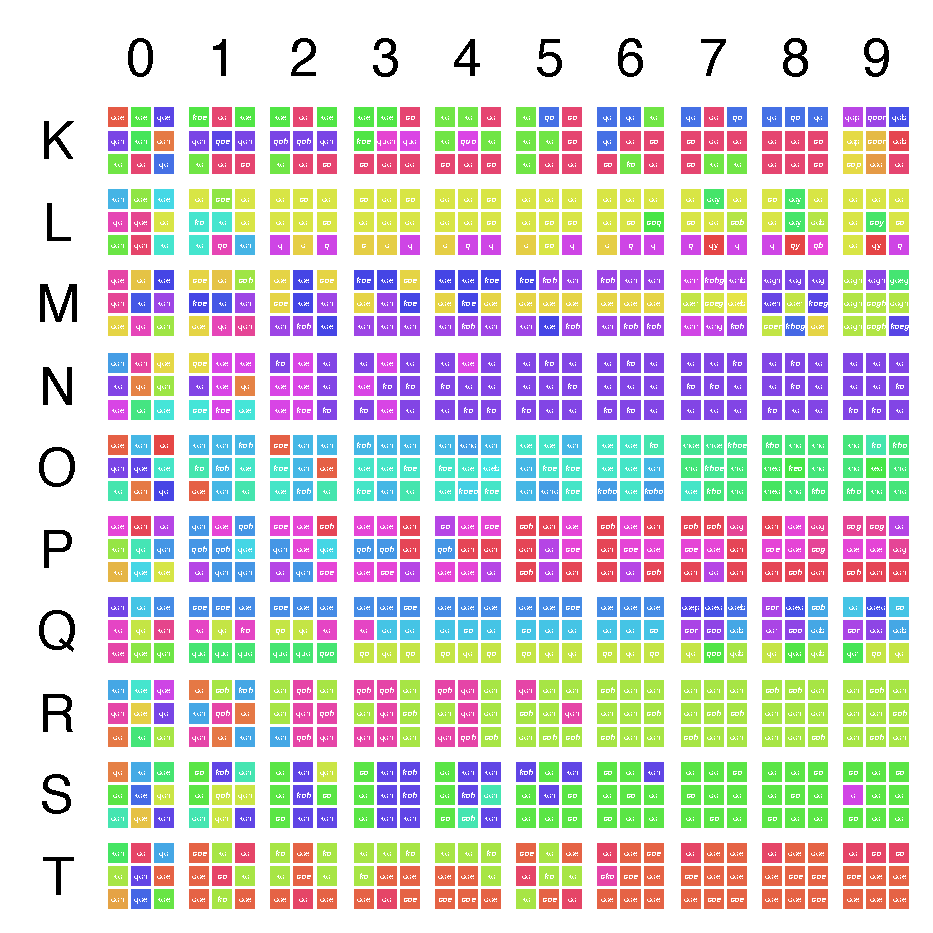
\includegraphics[]{figs/dif_com.eps}}
	\vspace*{2pt}
	\caption{Results from the Transmission~+ Communication condition in Experiment~1 (differentiation). Each matrix shows the suffix spelling system in use at a particular generation (shape on the rows, color on the columns, as in Fig.~\ref{stimuli}). Chains are labeled K--T and generations are labeled 0–9 (0 is the randomly generated seed system). Each chain uses an independent color palette, with each color representing a particular suffix spelling; similar colors indicate similar spellings. Spellings in bold-italic are the generalizations on unseen items. There are some isolated examples of differentiation through implicit generalization (K5, M1, P5, S2) and explicit innovation (K9, L7, M7, O4, Q7).}
	\label{dif_com}
	\end{figure}

The second type of color-expressive system is one that simply appropriates the expressive power of English to differentiate color: K9, M7, Q7, and to a lesser extent L7 and O4. In M7, for example, the participant added <r>, <g>, and <b> (presumably red, gold, blue) to the ends of the words, although the participant's partner only reciprocated the <g> spelling and seemingly failed to understand what was meant by <r> and <b>. In the case of Q7, the pair of participants added <r>, <o>, and <b> (presumably red, orange, blue) to communicate with high accuracy, but, although this system was retained into Generation~8, it started to disintegrate by Generation~9. Overall, in the five cases where English color letters were used, the systems did not really catch~on, perhaps because they retained spelling redundancy from the previous generation, resulting in unnecessarily complex suffix spellings that express both shape and color simultaneously. Q7, for example, uses <-coe->, <-co->, <-qo-> for shape plus <-r>, <-o>, <-b> for color. In addition to this handful of cases, there were a further four pairs of participants who used full English words as the suffix (typically <-pink> or <-red>, <-oran> or <-yell>, and <-blue>), but these pairs were excluded and replaced before iteration to the next generation.\footnote{In our preregistration, we stated that we would reject participants who used English color words. We allowed single letters because these were typically less transparent, especially in cases where the choice of letter (e.g., <g> or <r>) did not match how another person might have perceived the color (yellow vs.\@ gold vs.\@ orange or pink vs.\@ red). Indeed, as we see in the results, subsequent generations often did not pick~up~on the color letters (L9, M8, and Q9).} We mention these cases, however, because they are still examples of a conscious effort to differentiate---something that never happened in the Transmission-only condition.

To analyze more formally what types of system tend to emerge under different conditions, we first designated four reference systems that are of particular interest: holistic,\footnote{Although we use the term holistic here, this category also encompasses compositional suffixes that express both shape and color in a systematic way (specifically, K9, M1, M7, and Q7).} expressive, redundant, and degenerate. These four typological categories may be positioned along a complexity/cost continuum in terms of the number of suffix forms they make use of and how these forms are conditioned on meaning, as illustrated in Fig.~\ref{}. The holistic system has nine unique forms that express both color and shape, the expressive and redundant systems have three unique forms that express either color (expressive) or shape (redundant), and the degenerate category has one unique form that expresses nothing. To classify a participant's output into one of these four categories, we compute which of the reference systems is most similar in terms of its information content. To do this, we formalize the systems as set partitions (i.e., a partitioning of the universe of meanings into disjoint subsets) with variation of information \parencite[VoI;][]{Meila:2007} defined as the distance metric between any two such partitions.\footnote{VoI is a proper metric on set partitions, measuring the amount of information (in bits) that is lost and gained in the transformation of one set partition into another. Under this metric, the holistic and degenerate systems are considered very dissimilar because they carry very different levels of information content. The expressive and redundant systems are also considered very dissimilar because, although they carry the same amount of information, the information they carry is orthogonal (shape in the case of redundant, and color in the case of expressive).} Then, rather than simply classify a given system into exactly one typological category, we compute a probability distribution over the typological space according to the respective distances of the four reference systems. This gives a slightly more nuanced view of the typological distribution by accounting for cases where a given system might be partially suggestive of one typological category but also suggestive of another (e.g., T9 is part redundant, part degenerate). The typological probability distribution $t$ over the set of four reference systems $R$ was calculated for participant system $s$ according to% $t(i) \propto e^{-2\mathrm{VoI}(R_i, s)^2}$,
\begin{equation}
	t(i) \propto e^{-2 \cdot \mathrm{VoI}(R_i, s)^2}
\end{equation}
and averaged over chains for a given generation.

	\begin{figure}
	\makebox[\textwidth][c]{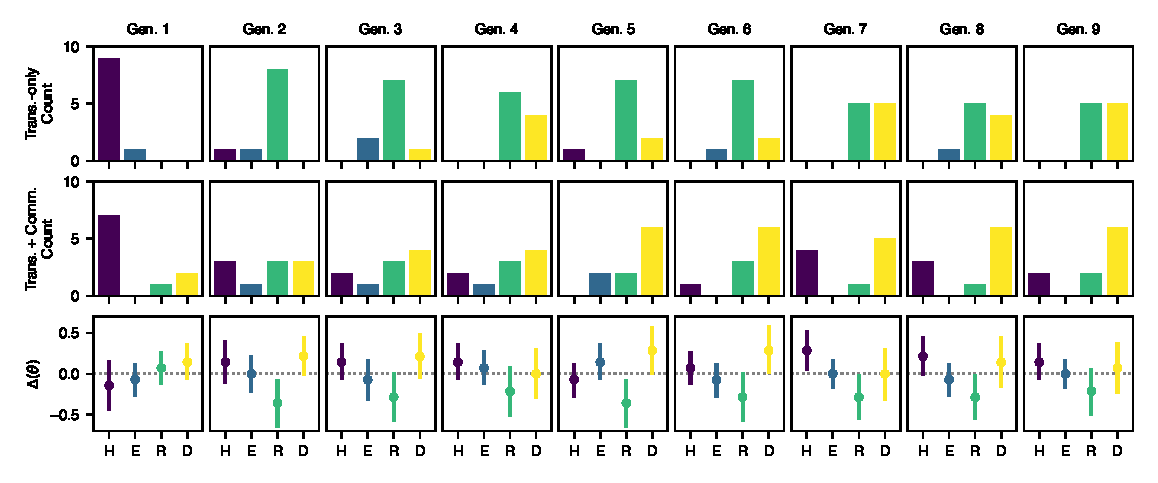
\includegraphics[]{figs/typ_dist_dif.eps}}
	\vspace*{2pt}
	\caption{Typological distribution at each generation and in each condition across four typological categories: holistic (H; purple), expressive (E; blue), redundant (R, green), and degenerate (D; yellow). At Generation~0, all 10 chains in both conditions use a holistic system (by design). In Transmission-only, the systems switch first to a redundant and then to a degenerate patterning. In Transmission + Communication, the systems ultimately become degenerate, but also tend to favor holistic systems over redundant ones along the way. Expressive systems were rare in both conditions.}
	\label{typ_dist_dif}
	\end{figure}

The results are plotted in Fig.~\ref{typ_dist_dif}. These probability distributions can be read as the proportion of chains that adopted each of the four configurations at each generation. At Generation~0, all chains are holistic by design. In Transmission-only, there is an initial rapid increase in the number of chains classified into the redundant typological category. The dominance of the redundant category is then gradually eroded as the chains transition to degeneracy. In Transmission + Communication, there is initially a fairly even mix of all four kinds of system, but by Generation~9, degenerate systems tend to be most common. There is, however, a notable increase in holistic systems emerging in later generations; these are the cases of compositional suffixes that arose through the addition of English color letters on top of redundant suffix spellings.

As a quantitative measure of how informative the orthographic systems are over time, we adopt communicative cost \parencite{KempRegier:2012, Regier:2015, Kemp:2018}. Communicative cost expresses how much information is lost, on average, when a speaker/writer attempts to convey a meaning to a listener/reader using some shared signaling system. If the system contains no ambiguities (all meanings are expressed by unique signals), communicative cost will be zero---that is, zero information will be lost during each attempt to communicate using that system. Communicative cost will take some larger value if the system contains ambiguity. Formally, it is given by% $\sum_{m \in U} \mathrm{Pr}(m) ( -\log \mathrm{Pr}(m|s_m) )$,
	\begin{equation}
	\sum_{m \in U} \mathrm{Pr}(m) ( -\log \mathrm{Pr}(m|s_m) ),
	\end{equation}
where $U$ is the universe of meanings that may be expressed, $\mathrm{Pr}(m)$ is the probability that a particular meaning would need to be expressed, and $\mathrm{Pr}(m|s_m)$ is the probability that a reader would infer meaning $m$ given that a writer produced signal $s$ for meaning $m$. In our case, $U$ is the set of nine alien objects, $\mathrm{Pr}(m)$ is set to $1/|U|$ (all objects need to be talked about with equal probability), and $\mathrm{Pr}(m|s_m)$ is given by $1/|M_s|$, where $M_s$ is the set of meanings labeled $s$ according to the system.

	\begin{figure}
	\makebox[\textwidth][c]{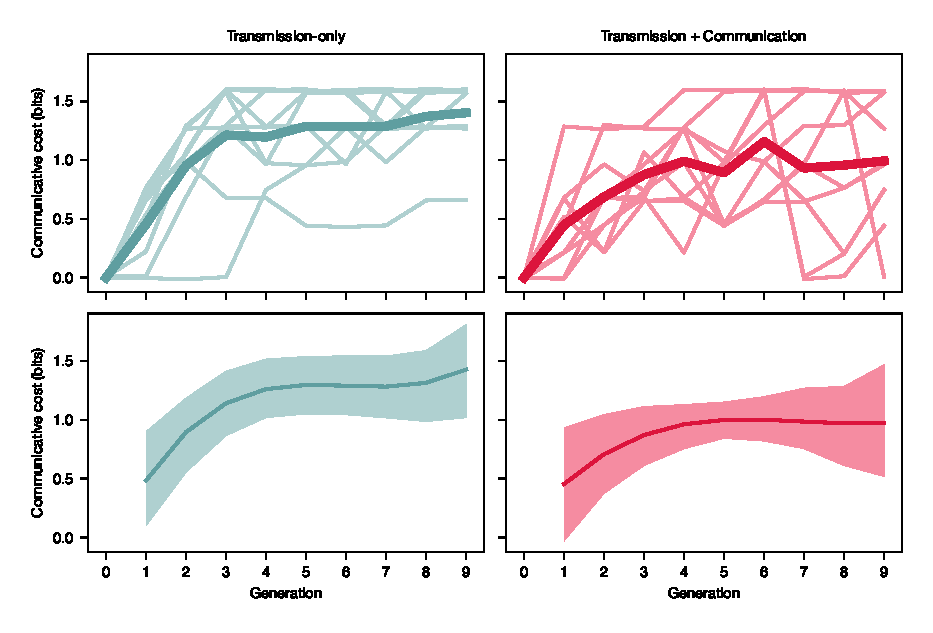
\includegraphics[]{figs/cost_dif.eps}}
	\vspace*{2pt}
	\caption{Communicative cost by generation under Transmission-only (blue) and Transmission + Communication (red). The upper panels show each individual transmission chain (thin lines; with jitter) and the mean across chains (thick lines). The lower panels show a polynomial regression model of the data (posterior mean and 95\% HDI). Generation~0 is not included in the model, since it does not represent participant data.}
	\label{cost_dif}
	\end{figure}

Fig.~\ref{cost_dif} plots communicative cost over the nine generations of cultural transmission in each condition. In the upper panels, each thin line represents an individual transmission chain, and the thick lines shows the mean across chains. The initial, generation-0 seed systems are all fully informative (zero cost) because each meaning is signaled by a unique arbitrary spelling. In both conditions, cost increases with generation, implying that the languages become less informative over time. This is to be expected in the Transmission-only condition, since there is only pressure from learnability, so the systems evolve to become simple and transparent. In contrast, this is not the expected result in Transmission + Communication, where the communicative pressure should promote the emergence of informative systems. This result does, however, align with our qualitative interpretation of the data, which suggested that participants in the communicative condition rarely produced differentiated spellings, be it through explicit innovation or implicit generalization. Interestingly, however, cost plateaus at around 1.3~bits in Transmission-only and around 1~bit in Transmission + Communication, suggesting that there is some tendency for the systems to remain slightly more informative in the communicative condition.

	\begin{figure}
	\makebox[\textwidth][c]{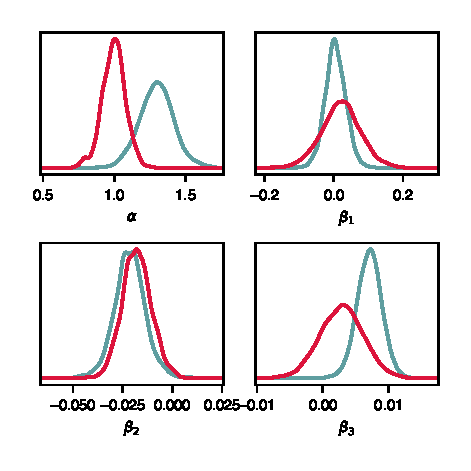
\includegraphics[]{figs/posterior_dif.eps}}
	\vspace*{2pt}
	\caption{Posterior parameter estimates for the Experiment~1 polynomial regression model. Blue curves show results for the Transmission-only condition and red curves show results for the Transmission + Communication condition. $\alpha$ represents the intercept of the polynomial (Generation~5) and the $\beta$ parameters characterize its shape.}
	\label{posterior_dif}
	\end{figure}

To evaluate this argument statistically, we regressed cost on generation in a Bayesian, hierarchical, polynomial regression model. The posterior parameter estimates are shown in Fig.~\ref{posterior_dif}. Essentially, the $\beta$ parameters of the model (characterizing the shape of the polynomial) do not differ substantially between conditions, but the intercepts ($\alpha$) do appear to differ. Since generation was centered (for the purpose of fitting the model), the $\alpha$ parameters correspond to Generation~5 and therefore represent the main plateaus of the polynomials. The posterior difference between $\alpha_\mathrm{tran}$ and $\alpha_\mathrm{comm}$ was 0.301~bits (95\%~HDI: 0.014--0.597). This difference, and its credible interval, is greater than zero, pointing to an effect of condition on the level at which cost plateaus. We emphasize, however, that this difference represents a relatively small effect size, corresponding to a 9.4 percentage point advantage for systems that emerged in the communicative condition (i.e., systems that emerged under Transmission-only would, on average, yield a communicative success rate of 40.7\%, whereas the equivalent value for Transmission + Communication is 50.1\%). Thus, although the presence of the communicative pressure does appear to make a difference to the informativeness of the emergent systems, that difference is not especially impressive considering that an ideal, expressive system of suffix spellings would support a 100\% success rate.

\subsection{Summary}

Our first experiment tested the ability of the differentiation model to explain the emergence of an informative, heterographic orthography, but we found little evidence of systematic orthographic differentiation. Exposed to an orthography with high variation, learners could have gradually conditioned that variation on the dimension where it would have been useful from the point of view of disambiguation, color, yielding differentiated forms in the orthography. But this did not happen, even under communicative pressure. Instead, when spelling variation was conditioned on anything, it was conditioned on shape, resulting in redundant suffix spellings. This result is in stark contrast to most prior experimental iterated learning studies, in which informative, compositional systems do typically emerge, especially under communicative pressure. So, what was different about the present experiment? The primary difference was the presence of a spoken language that is decidedly \textit{not} informative, which acts as a cue to participants that the language does not mark color and that, therefore, the orthography should not mark color. Faced with variation that could be conditioned on shape or color, learners rule out the possibility that it might be conditioned on color, since such a hypothesis would be in conflict with the spoken language. As a result, variation in spelling comes to be associated with particular stems, resulting in the emergence of idiosyncratic suffix spellings that serve no real purpose. A rough analog of this redundancy can be found in English in the spelling of /-ʃən/ (<cian>, <sion>, <ssion>, or <tion>), which is largely conditioned on the stem (e.g., \textit{magician}, \textit{expansion}, \textit{transmission}, and \textit{invention}).

Another pathway through which differentiation could have occurred is through conscious innovation, especially in the communicative conditions, where participants could have increased their bonuses substantially by innovating a system of color markers. However, there was no evidence of such innovation, and only four participants mentioned that they even \textit{considered} this possibility in their post-test comments (e.g., ``I wondered if I should use the color suffix rule even where I did not think it was the right word to try and help my partner get the right color object''). Why do participants choose not to innovate or even regularize an imperfect system? Firstly, although innovation was not expressly forbidden, it was perhaps suggested by the overall structure of the experiment that we expected them to use the orthography learned during training. Participants who adopted this interpretation may have feared diverging from their training either because they themselves wanted to avoid breaking the rules or because they did not know whether their partner would feel comfortable breaking the rules. Secondly, even if participants are willing to diverge, they are presented with an alignment problem: How can they decide what system of color marking to use when there is no channel through which they can have a meta-discussion? They can only use trial-and-error, and even then, the process is complicated by participants simultaneously adapting to each other's systems. Interestingly, these are dynamics that also exist in the real world, where deviation from received, sacrosanct spellings is considered socially unacceptable or uneducated (e.g., the non-standard spelling <thru> has struggled for decades---or perhaps centuries---to make any headway against <through>), and even under more progressive attitudes to change and innovation, the problem of achieving community buy-in remains, especially when the change is not imposed by top-down authority: If I decided to start using the spelling <banque> to differentiate the financial institution from river banks, would anyone take my spelling seriously or even understand the distinction I was trying to make?

Overall, our first experiment suggests that differentiation---be it through a self-organizing process in learning or through a conscious process of innovation in use---is not a good model of heterography, unless enforced by top-down authority. We now turn to consider the conservation model.

%~%~%~%~%~%~%~%~%~%~%~%~%~%~%~%~%~%~%~%~%~%~%~%~%~%~%~%~%~%~%~%~%~%~%~%~%~%~%~%~%~%~%~%~%~%~%~%~%~%~%~%

\section{Experiment 2}

We now turn our attention to the conservation model of heterographic homophones: Given that an informative system already exists (both in speech and in writing), does that informative system persist in writing even after the spoken language has degenerated into homophony? And, importantly, does this happen preferentially in the presence of a communicative pressure?

\subsection{Methods}

The methods were identical to Experiment~1 with two main exceptions: The artificial language used to seed each chain started out fully compositional (in both its spoken and written forms), and two sound mergers were artificially induced during cultural transmission, resulting in the spoken forms of the suffixes becoming increasingly uninformative over time.

\subsubsection{Participants}

The experiment was completed by 297 native-English participants recruited through Prolific. The payment and bonusing scheme was identical to Experiment~1 (median bonus: £0.78). The median completion time was 15~m with a median hourly rate of £7.99 (£10.68 including bonus). 17 participants were excluded because they (or their partners) failed the auditory attention checks (15) or used English color words (2). A further 10 participants were lost to communication-game pairing failures. Like Experiment~1, the final dataset comprises 270 participants: 90 in the Transmission-only condition (10 chains of 9 subjects) and 180 in the Transmission~+ Communication condition (10 chains of 9 pairs of subjects).

\subsubsection{Stimuli}

The alien objects and word stems were identical to Experiment~1. Unlike Experiment~1, however, the transmission chains were seeded with a fully compositional language that uses three distinct suffixes to systematically express each of the colors. A separate set of suffixes was created for each chain by concatenating a randomly drawn consonant from \{/f/, /s/, /ʃ/\} and a randomly drawn vowel from \{/ə/, /ɛɪ/, /əʊ/\}, both without replacement. For example, one chain might use the suffixes /fəʊ/, /ʃə/, /sɛɪ/, while another chain might use /sə/, /fɛɪ/, /ʃəʊ/. The initial orthographic system was transparent and based on the following phoneme–grapheme mapping: \{/f/→<f>, /s/→<s>, /ʃ/→<x>, /ə/→<a>, /ɛɪ/→<ei>, /əʊ/→<oe>\}. The suffixes were designed to be distinctive (and therefore easy to memorize and associate with colors), but also similar enough to (mostly) allow for somewhat plausible sound mergers and result in somewhat plausible spellings following sound merger (e.g., it is plausible that /f/ might supplant /s/ or /ʃ/ in speech or that /ʃ/ might be spelled <s> or <x> in writing). We attempted to achieve this balance by combining consonants that are very similar with vowels that are very dissimilar, while also avoiding reuse of any sounds present in the stems. The spoken forms were synthesized using the Apple text-to-speech synthesizer (Moira voice).

\subsubsection{Sound change}

	\begin{figure}
	\makebox[\textwidth][c]{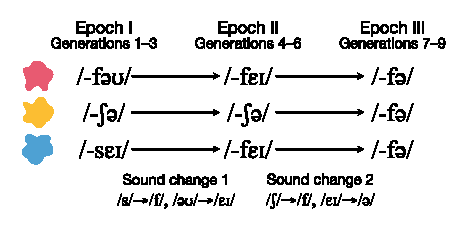
\includegraphics[]{figs/sound_change.eps}}
	\vspace*{2pt}
	\caption{Examples of the spoken suffixes in Experiment~2. During Epoch~I, color is represented by three distinct spoken suffixes. During Epoch~II, two of the suffixes are homophonous, reducing the informativeness of the spoken language. During Epoch~III, the spoken form of the language makes no color distinction.}
	\label{sound_change}
	\end{figure}

As in Experiment~1, each transmission chain was run for nine generations. Additionally, the nine generations were divided into three epochs, each lasting three generations. During Epoch~I (Generations~1 to~3), the three spoken suffixes were distinct (as described above), allowing the spoken language to express all three colors without ambiguity. During Epoch~II (Generations~4 to~6), the spoken language had two distinct suffix forms, reducing its informativeness. During Epoch~III (Generations~7 to~9), all three spoken suffixes were homophonous, just as in Experiment~1, making the spoken language entirely uninformative about color. This was achieved through two sets of sound changes, the first occurring in the transition from Epoch~I to~II and the second occurring in the transition from Epoch~II to~III. An example is illustrated in Fig.~\ref{sound_change}. In the first sound change, two of the spoken suffix forms were chosen at random and the consonant from one (chosen at random) was paired with the vowel from the other, resulting in a new suffix form that replaced the original two. In the second sound change, the remaining two suffix forms were merged in the same way, resulting in full homophony. Crucially, the spellings do not automatically change following a sound change event; rather, the orthographic system is free to adapt (or not) in response to the sound changes. Note also that an individual participant does not directly experience the sound changes; rather, a Generation~4 participant, for example, would always hear Epoch~II sounds, while observing spellings produced by a Generation~3 participant (presumably representing the Epoch~I sounds). In reality, of course, sound change is more gradual, with individual speakers experiencing both outgoing and incoming spoken forms within their lifetimes.

\subsection{Results}

	\begin{figure}
	\makebox[\textwidth][c]{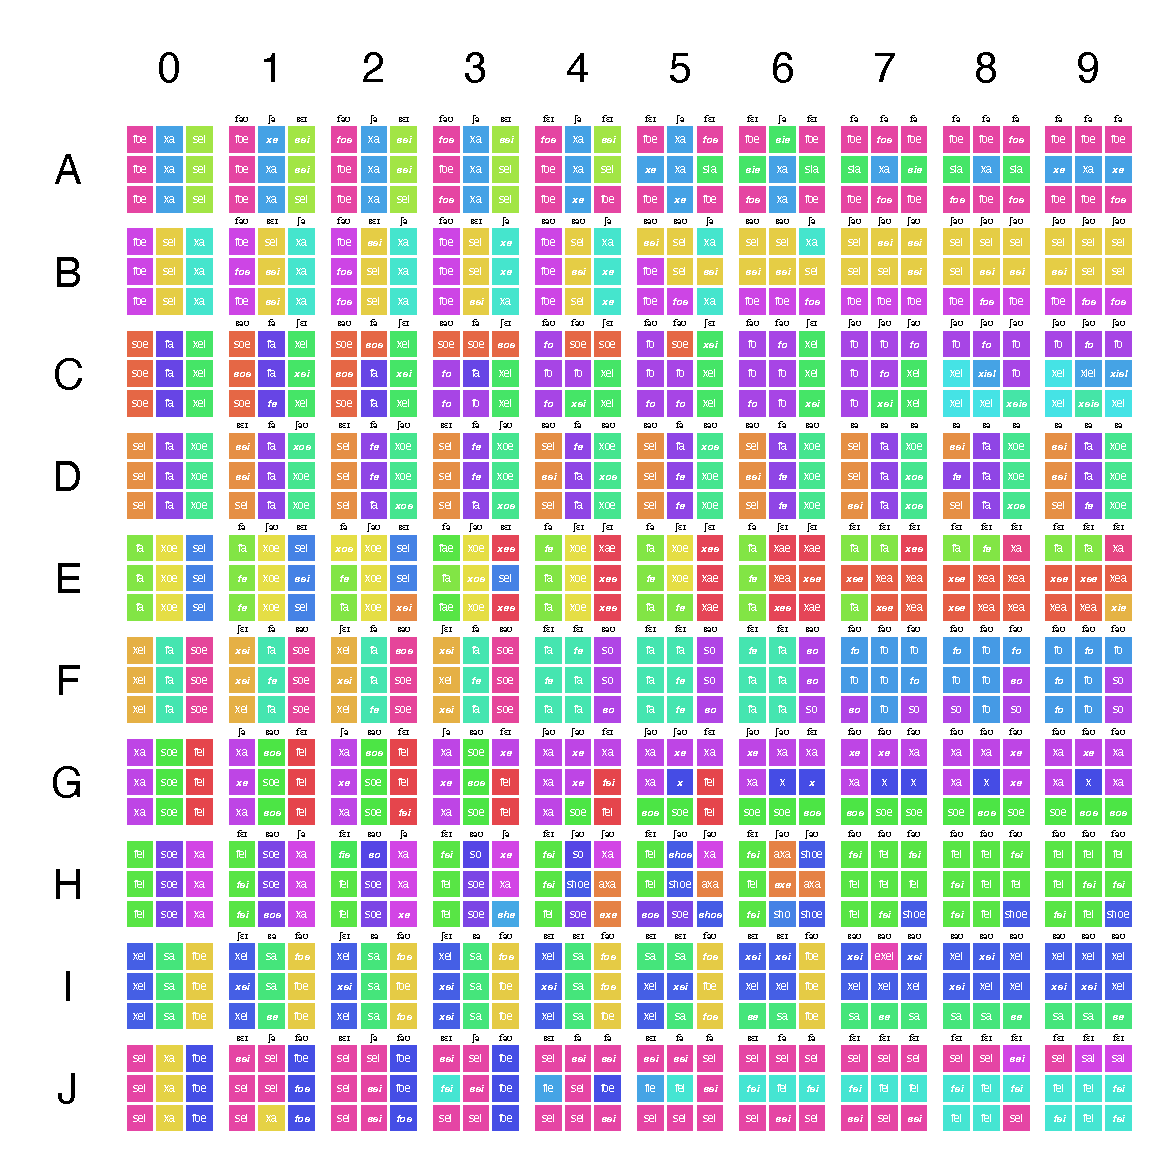
\includegraphics[]{figs/con_lrn.eps}}
	\vspace*{2pt}
	\caption{Results from the Transmission-only condition in Experiment~2 (conservation). Each matrix shows the suffix spelling system in use at a particular generation (shape on the rows, color on the columns, as in Fig.~\ref{stimuli}). Chains are labeled A--J and generations are labeled 0–9 (0 is the randomly generated seed system). Each chain uses an independent color palette, with each color representing a particular suffix spelling; similar colors indicate similar spellings. Spellings in bold-italic are the generalizations on unseen items. The final systems are characterized by the conservation of form without the conservation of expressivity.}
	\label{con_lrn}
	\end{figure}

The results for all ten chains (labelled A--J) in the Transmission-only condition are shown in Fig.~\ref{con_lrn}. It is immediately clear that color-expressive suffixes (as indicated by vertical stripes) are maintained fairly reliably through the first epoch; perfectly in the case of Chains~A, B, D, F, and~I, and with some errors in the other five chains. Some of these errors are very minor, such as the use of <sha> instead of <xa> for one item in H3, while others are more catastrophic, such as the early loss of the <sei>/<xa> distinction in Chain~J. Generation~4 represents the first real test of the orthographic systems in the face of sound change, and, in most cases, the Generation~3 systems are preserved quite faithfully (Chains~A, B, D, E, H, and~I), but by the end of the epoch (Generation~6), many have degenerated into redundant systems that encode shape (Chains~B, G, and~J) or transparent systems that mirror the Epoch~II pattern of homophony (Chains~C, E, F, and~I). These processes continue into Epoch~III and by the ninth generation, all systems have become degenerate, redundant, or some mixture of the two. The one exception is Chain~D, whose original spellings---<sei>, <fa>, <xoe>---were conserved perfectly through to the final generation with only one generalization error in Generation~8, which was quickly reverted in Generation~9.

Like Experiment~1, redundant systems are characteristic of the Transmission-only condition, especially in Epoch~III. As the spoken suffixes becomes more homophonous, the variant spellings are increasingly conditioned on shape rather than color, perhaps because the spoken language signals to learners that the language does not mark color, so they rationalize the system as three words with idiosyncratic spellings. Interestingly, however, all chains exhibited conservation of spelling \textit{form}, even if the way in which spelling was conditioned on meaning was lost. For example, Chain~A ultimately represents the sound /fə/ with the spellings <foe> and <xa>, spellings that are internally inconsistent and contrary to standard uses of the Roman alphabet, but which trace their origins back to the original seed orthography. Overall, then, the Transmission-only condition in Experiment~2 is characterized by the conservation of spelling \textit{form} without the conservation of expressivity.

	\begin{figure}
	\makebox[\textwidth][c]{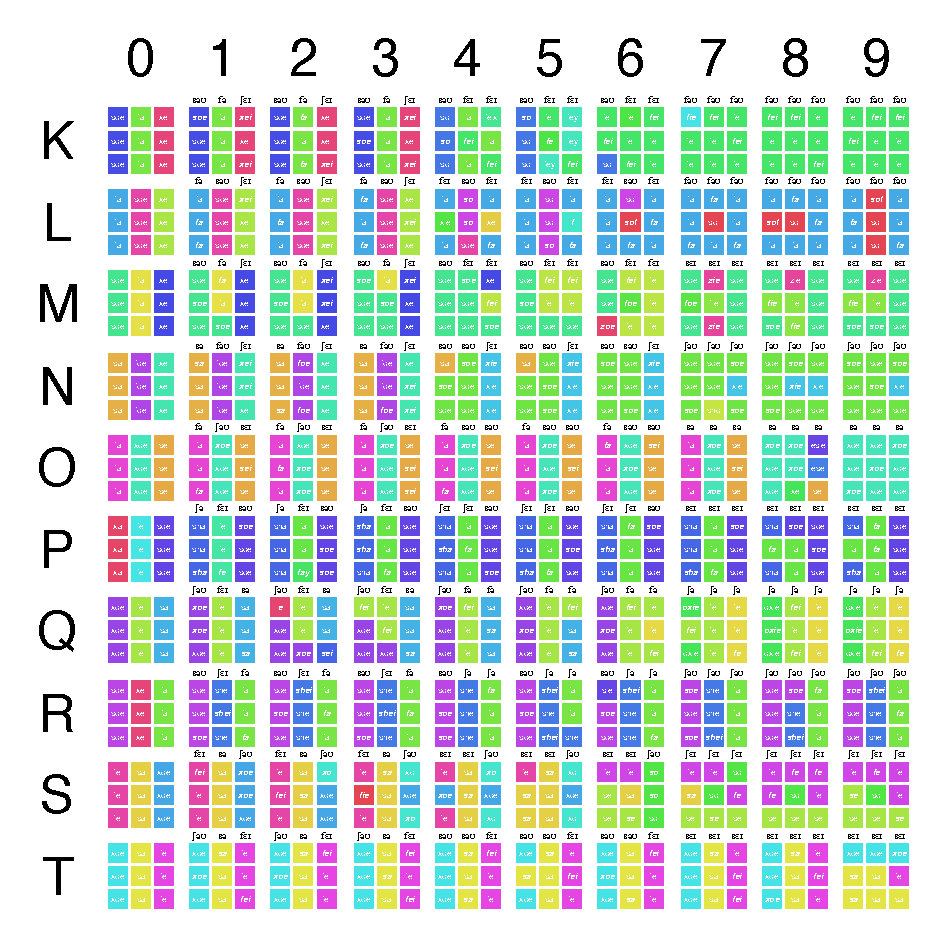
\includegraphics[]{figs/con_com.eps}}
	\vspace*{2pt}
	\caption{Results from the Transmission~+ Communication condition in Experiment~2 (conservation). Each matrix shows the suffix spelling system in use at a particular generation (shape on the rows, color on the columns, as in Fig.~\ref{stimuli}). Chains are labeled K--T and generations are labeled 0–9 (0 is the randomly generated seed system). Each chain uses an independent color palette, with each color representing a particular suffix spelling; similar colors indicate similar spellings. Spellings in bold-italic are the generalizations on unseen items. Five chains (O, P, Q, R, T) remain fully expressive into the final epoch, in most cases conserving the original forms.}
	\label{con_com}
	\end{figure}

The results for the Transmission~+ Communication condition (Chains~K--T) are shown in Fig.~\ref{con_com}. Like Transmission-only, the seed systems are mostly maintained faithfully through Epoch~I; perfectly in the case of Chains~K, L, N, O, and~J, and with some errors in the other five chains, although some of these errors are non-destructive changes, such as <x> being replaced with <sh> in R1. Several systems were then maintained through Epoch~II, notably Chains~O, P, R, and~T, and, in one case, through to the end of Epoch~III (Chain~R, albeit with the original <xei> spelling replaced with <shei>). The Chain~O system was preserved up to Generation~7, Chain~P was maintained up to Generation~7 and almost to Generation~9 with two modifications (<sha> instead of <xa> and <fa> instead of <fei>), and Chain~T was conserved faithfully up to Generation~8. The final form of Chain~Q was also fully expressive, albeit through a combination of both conservation and differentiation: The <fei> form was conserved from the seed orthography, the <oxie> spelling appears to derive from a misremembering of <xoe> (partial conservation), and the <fe> spelling, which began as a typo introduced in Q6, seems to have been generalized across the blue items in Q7, perhaps to differentiate them from the yellow items (indeed, the participant's partner made the same generalization). A similar case of differentiation might also have occurred in L9, where the <sol> spelling (originally a typo on <so>) was generalized across the yellow items, resulting in a semi-expressive system (although the participant's partner generalized the <sol> spelling across shape).

Unlike Experiment~1, no participant pairs attempted to use English color letters and there was only one case of a pair using English color words in Generation~9 of Chain~K, although this pair was excluded and replaced (this generation was the only case in which the training input was fully degenerate, which would have resulted in a strong pressure to find a communicative solution in the form of English). Presumably, the general conservation of expressive spelling in Experiment~2 negated the need to innovate novel systems.

	\begin{figure}
	\makebox[\textwidth][c]{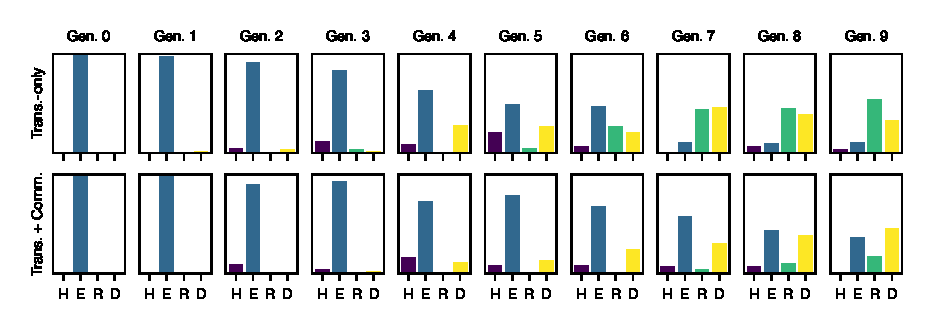
\includegraphics[]{figs/typ_dist_con.eps}}
	\vspace*{2pt}
	\caption{Typological distribution at each generation and in each condition across four typological categories: holistic (H; purple), expressive (E; blue), redundant (R, green), and degenerate (D; yellow). At generation~0, all 10 chains in both conditions use an expressive system (by design). In Transmission-only, the systems tend to transition to the redundant or degenerate patterning, while in Transmission + Communication, they tend to remain expressive for longer and disfavor the redundant pattern.}
	\label{typ_dist_con}
	\end{figure}

As in Experiment~1, we plot communicative cost by generation in both conditions (see Fig.~\ref{cost_con}). Each colored line represents an individual chain, and the thick black lines shows the mean across chains. These mean lines reveal a fairly clear effect from epoch. During Epoch~I, there is a shallow increase in cost with generation in both conditions. This represents a kind of baseline level of noise when the spoken languages are fully informative. During Epoch~II, there is a steep rise in cost in the Transmission-only condition, but a relatively shallow rise in Transmission + Communication. This is because the communicative pressure acts to slow down the rate at which the systems become transparent or redundant. In Epoch~III, the cost curve plateaus in the Transmission-only condition because the written languages have become sufficiently simple to be reliably learned and reproduced with little change. In Transmission + Communication, by contrast, the curve gets a little steeper because the systems still have some room to simplify and the pressure to simplify has been ramped up.

	\begin{figure}
	\makebox[\textwidth][c]{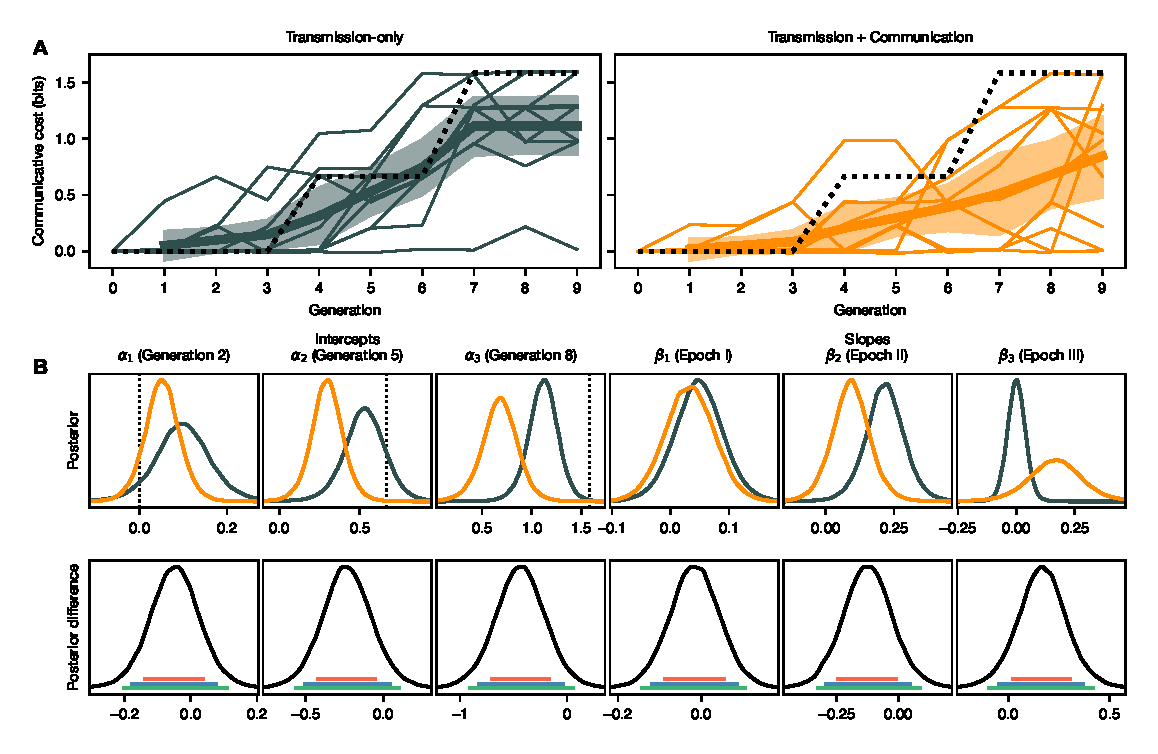
\includegraphics[]{figs/cost_con.eps}}
	\vspace*{2pt}
	\caption{Communicative cost by generation under Transmission-only (blue) and Transmission + Communication (red). The upper panels show each individual transmission chain (thin lines; with jitter) and the mean across chains (thick lines). The lower panels show a polynomial regression model of the data (posterior mean and 95\% HDI). Generation~0 is not included in the model, since it does not represent participant data.}
	\label{cost_con}
	\end{figure}

\subsection{Summary}

In contrast with Transmission-only, where only one chain remained expressive into Epoch~III, in Transmission~+ Communication, five chains (O,~P, Q, R, and~T) remained expressive, or six if you include Chain~B, whose <sol> spelling does find its origin in the <soe> spelling from the seed orthography.

%~%~%~%~%~%~%~%~%~%~%~%~%~%~%~%~%~%~%~%~%~%~%~%~%~%~%~%~%~%~%~%~%~%~%~%~%~%~%~%~%~%~%~%~%~%~%~%~%~%~%~%

\section{Discussion}

%~%~%~%~%~%~%~%~%~%~%~%~%~%~%~%~%~%~%~%~%~%~%~%~%~%~%~%~%~%~%~%~%~%~%~%~%~%~%~%~%~%~%~%~%~%~%~%~%~%~%~%

\section{Acknowledgments}

\noindent This work was funded by a grant from the Leverhulme Trust.

\printbibliography

\end{document}